\section{The Motivation of Multi-Messenger Astronomy}

The previous five chapters of this thesis have demonstrated the capabilities of the gravitational wave detectors and searches and how the field of gravitational wave astronomy has observed events which had previously never been seen. This chapter will cover how gravitational wave astronomy can be paired with traditional electromagnetic astronomy which has been the foundation of astronomy for thousands of years. There are specific events which can be observed with both gravitational waves and electromagnetic radiation, these are some of the most energetic events in our Universe such as the supernova of nearby stars and the kilonova from the merger of two neutron stars. An astrophysical event whose gravitational wave and electromagnetic emission has been detected is called a multi-messenger event.

Multi-messenger astronomy combines the information produced by the independent observations of the same event to understand more about the event itself. The Hubble constant is a measurement of the rate of expansion of the Universe and can be determine from electromagnetic radiation in two ways: from large scale cosmological measurements of the cosmic microwave background and, by using the astrophysical standard candle Cepheid variable stars. Gravitational waves can be used as another measurement of the Hubble constant.

The Hubble constant can be calculated using the very simple relation,
%
\begin{equation}
    cz = H_{0} D_{L}, 
\end{equation}
%
where $c$ is the speed of light, $z$ is redshift, $H_{0}$ is the Hubble constant and $D_{L}$ is the luminosity distance. We can take a gravitational wave event, such as a binary neutron star merger, and as long as we know the redshift and the luminosity distance we can calculate the Hubble constant.

The luminosity distance of a gravitational wave is proportional to the amplitude of the strain,
%
\begin{equation}
    h(t) \propto \frac{1}{D_{L}} , 
\end{equation}
%
which is obtained through gravitational wave searches and parameter estimation. The strain amplitude does have a degeneracy with the inclination angle of the binary neutron star system,
%
\begin{equation}
    h(t) \propto \sqrt{(1+\cos^{2}\iota^){2} + (2\cos\iota)^{2}},
\end{equation}
%
which is the angle between the line of sight to the observer and the orbital angular momentum of the source, affecting both the gravitational wave polarization and the amplitude. This means a source than is closer but edge-on, $\iota = 90^{\circ}$, can produce a similar amplitude to a source further away but face-on, $\iota = 0^{\circ}$. The inclination angle is very difficult to measure with the current detectors.

The redshift of a gravitational wave signal also has a degeneracy with the chirp mass of the source,
%
\begin{equation}
\mathcal{M} = \frac{(m_1 m_2)^{\frac{3}{5}}}{(m_1 + m_2)^{\frac{1}{5}}}.
\end{equation}
%
The frequency evolution of the signal is dependent on the chirp mass,
%
\begin{equation}
f(t) \propto \mathcal{M}^{\frac{5}{8}}t^{-\frac{3}{8}},
\end{equation}
%
which is directly measured from the gravitational wave signal but will undergo redshifting as it travels to the detectors. Therefore we would require a measurement of the Hubble constant in order to determine the correct amount of redshifting happening to the signal. Using an accompanying electromagnetic emission from an event, a kilonova from a binary neutron star system, we can locate the host galaxy of the source and therefore the redshift for the source.

We have a luminosity distance measured by the gravitational wave signal and a redshift measured by the electromagnetic observation and we can make a new estimation of the Hubble constant. Electromagnetically bright gravitational wave sources can be used as another standard siren for measuring the Hubble constant, highlighting the importance of observing multi-messenger events.

\section{GW170817}

Multi-messenger events are seen via a gravitational wave signal and then multiple electromagnetic signals from across the electromagnetic spectrum. We have observatories around the globe and in space which span this entire spectrum and can observe counterparts to our gravitational wave signal in all of the different frequency ranges: from high frequency gamma rays to long wavelength radio waves. The gravitational wave emissions of a merger event are seen before any optical emissions due to the inspiral of the binary system emitting detectable gravitational waves prior to the merger.

GW170817~\cite{GW170817:2017} is the first and only multi-messenger event observed, the Q-scan of which can be seen in figure~ADD and the GCN circular can be found at: \href{https://gcn.gsfc.nasa.gov/other/G298048.gcn3}{https://gcn.gsfc.nasa.gov/other/G298048.gcn3}. On the 17th August 2017 at precisely 12:41:04 UTC the gravitational waves from the merger of a binary neutron star system were seen by LVK detectors. Only $1.7$ seconds later a gamma-ray burst was seen by Fermi~\cite{Fermi:2022, Fermi_GW170817:2017} and INTEGRAL~\cite{INTEGRAL:2003, INTEGRAL_GW170817:2017}. The kilonova emissions were seen next, visual light by the Hubble Space Telescope (HST)~\cite{HST:2000, HST_GW170817:2021} at 11 hours, infrared by HST, VISTA~\cite{VISTA:2015, VISTA_GW170817:2017} and Spitzer~\cite{Spitzer:2004, Spitzer_GW170817:2018} at 12 hours and UV by Swift's UVOT~\cite{Swift:2004, Swift_GW170817:2017} at 15.3 hours post-merger. The final frequencies to be seen were X-rays by Chandra~\cite{Chandra_GW170817:2017} at 9 days post-merger and radio waves by VLA~\cite{VLA:2019, VLA_GW170817:2017} at 16 days post-merger. 

Analysing GW170817's gravitational wave signal and electromagnetic emissions reveal a binary neutron star system located in the Hydra constellation belonging to the galaxy NGC 4993~\cite{NGC4993:1998}. From these measurements we infer a Hubble constant from $62$ to $107$ $km s^{-1} Mpc^{-1}$~\cite{GW170817_H0:2017}, not accurate enough to break the previous cosmological-astrophysical Hubble constant measurement tension. As we observe more electromagnetically bright events from which we can measure the luminosity distance we will be able to constrain the measured value of the Hubble constant.

\section{GW170817 in Early Warning}

In the future we might not get as lucky as we did with GW170817. Each electromagnetic frequency has different timing windows in which their telescopes can be pointed to observe the event. Fermi detected GW170817 $1.7$ seconds after the merger and is capable of observing the whole sky with the exception of the region occluded by the Earth~\cite{Fermi:2022}, therefore, there is a portion of the sky it cannot view, meaning the initial confirmation of a multi-messenger event could be missed for a future electromagnetically bright event.

The gravitational wave signal from GW170817 was present in the LVK detectable frequency range for $60$ seconds, pre-merger had even occurred. If we detect events as soon as they appear then we can alert the international scientific community that a gravitational wave event was going to happen so they can be prepared. While $60$ seconds of warning might not be enough for Fermi to slew to a different part of the sky, as we improve our detectors we can increase the gap between detection and merger.

Sky maps are used to indicate the area on the sky which contains the most likely source location of the gravitational wave signal. We can improve the sky location with: more detectors at greater geographical distances and with different orientations improves triangulation and more sensitive detectors lead to better SNRs. Other things may also affect the sky localisation such as: the sky position, we are more sensitive to some parts of the sky; the antenna pattern of the detectors, the response of the detector depends on the relative angle of the incoming signal which changes as the Earth rotates. A better sky localisation leads to a more constrained, smaller area sky map.

GW170817 was seen by gravitational wave searches and the initial alert to astronomers was sent $27$ minutes after merger time. The LIGO-Livingston data contained a nasty glitch which had to be removed before a sky map could be made, leading to a sky map latency of $5$ hours and $14$ minutes. The Q-scan containing the glitch can be seen in figure~ADD(reproduced from \cite{GW170817:2017}, figure 2) and the original event was uploaded to GraceDB (the Gravitational Wave Candidate Event Database) and can be seen here: \href{https://gracedb.ligo.org/events/G298048}{https://gracedb.ligo.org/events/G298048}.

We now have more robust and well tested search pipelines which are capable of finding gravitational wave events with a maximum latency of $20$ seconds post-merger~\cite{PyCBC_Live:2018}, with the ability to rapidly make sky maps using BAYESTAR~\cite{BAYESTAR:2016} and have the ability to auto-gate any loud glitches in the data. Assuming the BAYESTAR sky map is good enough and there are enough detectors to effectively cover the whole sky map (we have instruments such as GOTO which are used specifically for gravitational wave event followup~\cite{GOTO:2020}), gamma-ray bursts can arrive less than two seconds after the gravitational wave merger. This is not nearly enough time to produce a sky map or relocate a telescope. As an example, the PyCBC Live full-bandwidth gravitational wave search has a maximum latency between detection and upload to GraceDB of $20$ seconds, as shown by figure~\ref{6:fig:latency_plot}.
%
\begin{figure}
    \centering
    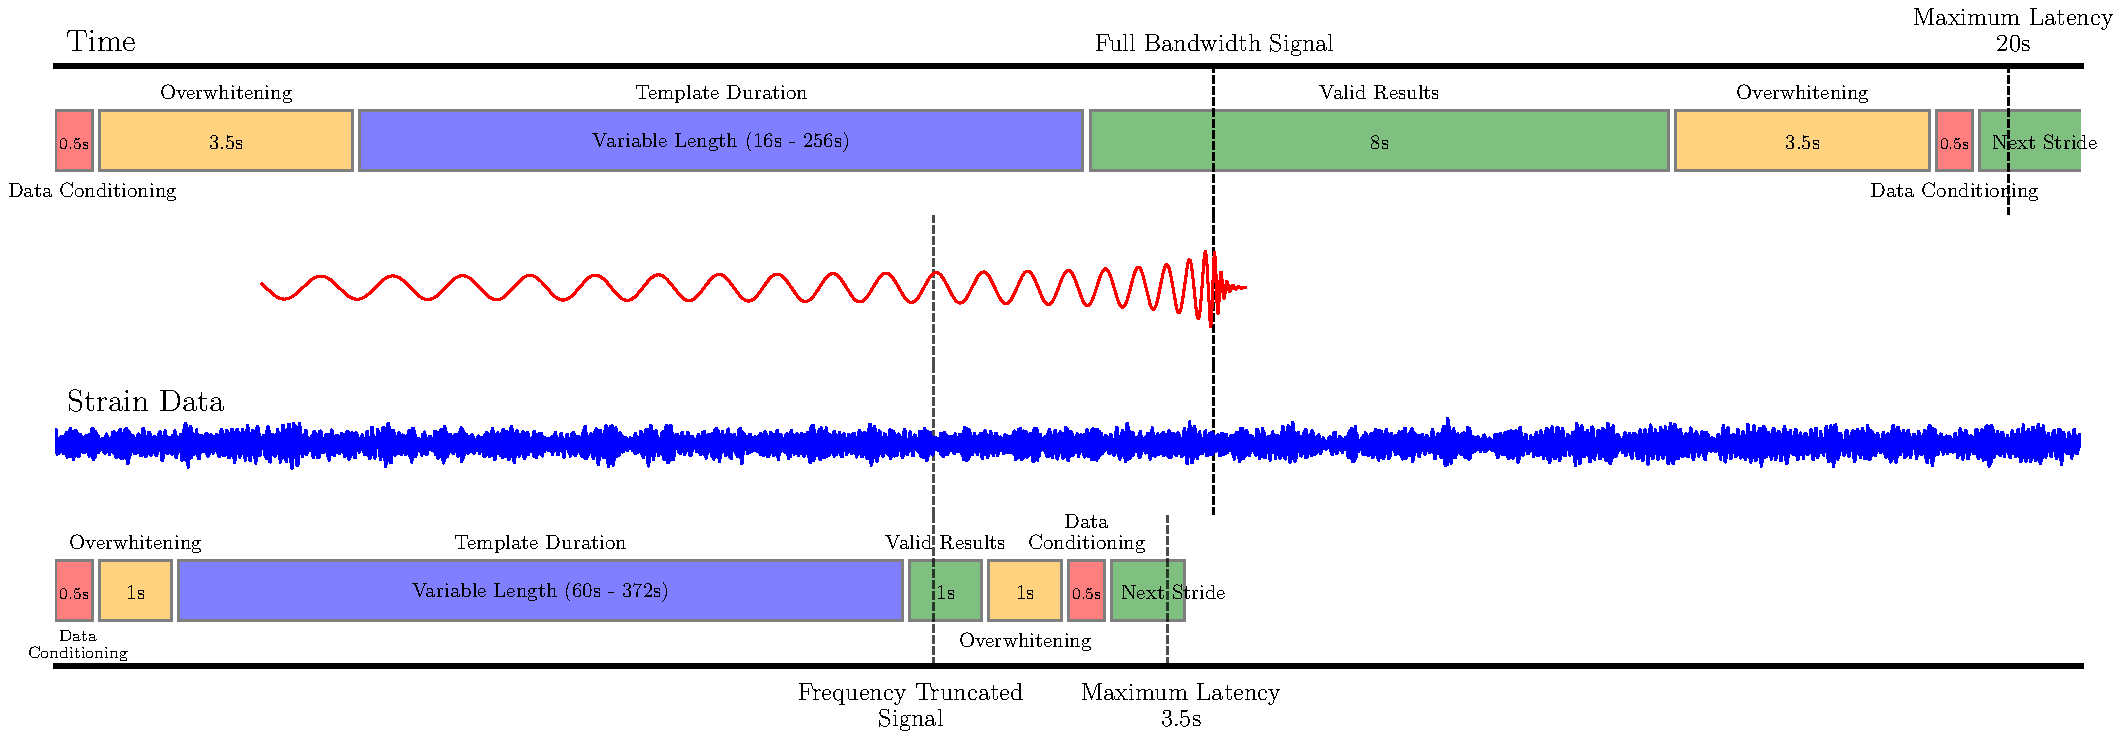
\includegraphics[width=\textwidth]{images/6_earlywarning/gw170817/latency_plot.pdf}
    \caption{}
    \label{6:fig:latency_plot}
\end{figure}
%
An early warning search will search for pre-merger gravitational wave signals. When one has been found it can estimate the time of coalescence, produce a sky map, and send out an alert to the international astronomy community to be prepared for an incoming gravitational wave merger. The details of the PyCBC Live early warning search will be covered in this chapter.

We can demonstrate the early warning search's efficacy on GW170817. When we search through the original data we observe the gravitational wave signal X seconds pre-merger. When we inject a GW170817-like signal into O4 data we see the signal X seconds pre-merger, representative of what we would see if GW170817 happened today. By implementing an early warning search in PyCBC Live we are capable of identifying gravitational signals before merger. This will aid in localising potentially electromagnetically bright gravitational wave signals and inform telescopes of all frequency ranges around the globe and in space to capture as much of the electromagnetic counterpart as possible, enabling greater quality multi-messenger astronomy.

\section{Early Warning Search}

PyCBC Live has two currently active configurations running on real gravitational wave data in real time: the full-bandwidth search aims to identify all gravitational wave signals in the data in low-latency; the early warning search aims to identify potentially electromagnetically bright signals prior to their merger.

The PyCBC Live full bandwidth and early warning searches use the same infrastructure and code. The full bandwidth search uses a data stride of eight seconds, meaning new data is loaded every eight seconds, while the early warning search has a data stride of one second. As shown in figure~ADD the full bandwidth search has a minimum latency of X seconds and a maximum latency of Y seconds between gravitational wave merger and PyCBC Live detection, the corresponding figure can be made for the early warning search, seen in figure~ADD, where we can see that we have a minimum latency between initial gravitational wave detection of -X seconds and a maximum latency of -Y seconds.

The clear difference between the two searches is the ability for the early warning search to detect gravitational wave signals prior to merger using templates which have been truncated a specific frequencies. When a significant amount of SNR has been accumulated in the inspiral region we can detect the signal and predict the time of merger, and with multiple templates for the same signal at different final frequencies we can build up a signal and report multiple events for the same gravitational wave signal. We are even able to make preliminary skymaps from these frequency truncated events, with the skymap becoming more and more accurate as more SNR is accumulated in higher final frequency events.

\section{Template Bank}

The PyCBC Live early warning search uses a frequency truncated template bank to search for gravitational wave signals prior to merger. The full bandwidth gravitational wave templates are generated with the \verb|TaylorF2| waveform model which models the inspiral region of the signals and is unable to accurately model the merger phase, this is acceptable because these low mass signals merge above the upper frequency band of detector sensitivity. The frequency evolution of the inspiral region of \verb|TaylorF2| waveforms is monotonic in time, meaning a specific time before merger corresponds directly to a particular frequency to truncate to. Therefore to observe a template $30$ seconds pre-merger, we can map that directly to a frequency and trunacate the template at that frequency. This is even easier when we consider that \verb|TaylorF2| waveforms are frequency domain so no conversion between time and frequency is required.

Initially the early warning search template bank was spaced to correspond to 5\% increments of the total expect SNR, leading to a template bank with truncated frequencies of \verb|30, 35, 40, 45, 50, 55, 60, 65| (IS THIS ACTUALLY TRUE? LOL?). The current bank we use has truncated frequencies of \verb|29, 32, 38, 44, 49, 56| which match the grid of frequencies used by the other early warning searches of the pipelines: GstLAL~\cite{GstLAL:2020}, MBTA~\cite{MBTA:2021} and SPIIR~\cite{SPIIR:2020}. These templates correspond to roughly \verb|60, 46, 29, 20, 15, 10| seconds before merger for a $1.4M_\odot$-$1.4M_\odot$ BNS signal. The bank is constructed by generating a template bank using the standard geometric placement algorithm (Brown et al. 2012 - FIND THE CITATION) and a minimal match of $0.97$ for each frequency cutoff and then combining the six template banks into one.

The template parameters themselves are chosen to represent potentially electromagnetically bright, low mass BNS or NSBH systems. This means that a single full bandwidth signal isn't simply generated and split into six frequency truncated templates and in fact a full bandwidth template might not have six frequency truncated templates that exactly match but they are covered by a nearby template with a minimum match of $0.97$. The masses of the two systems are limited between $1-3 M_\odot$, with no spins. The PSD used to generate the template bank is \verb|aLIGO140MpcT1800545| which is a representative PSD of (BLAH BLAH BLAH).

The complete early warning template bank is $9180$ templates, making for a very light weight search computationally when compared to the ~$700,000$ templates being used in the full bandwidth PyCBC Live search. Not only are there a smaller number of templates in the template bank, the templates themselves are shorter in duration when compared to their full bandwidth counterparts in the full bandwidth template bank. While low mass signals are typically very long in duration compared to high mass systems, due to existing in the sensitivity band of the detectors for longer, this is countered by the frequency truncation.
%
\begin{figure}
    \centering
    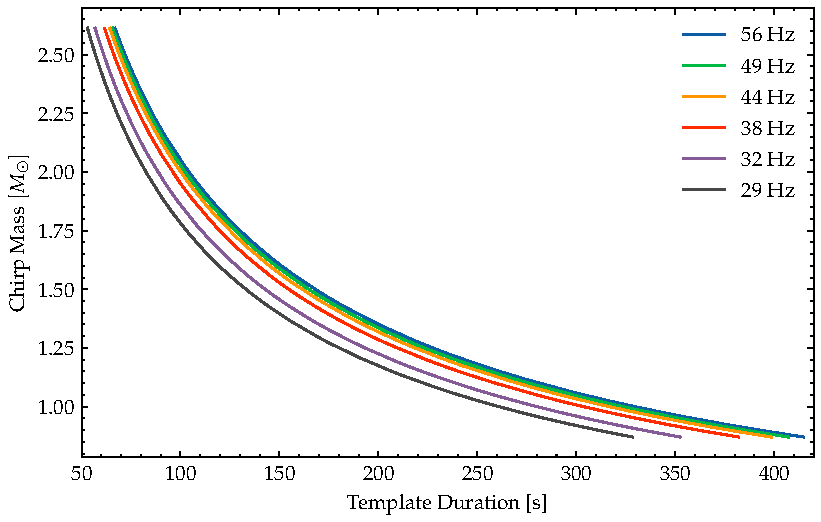
\includegraphics[width=\textwidth]{images/6_earlywarning/search/template_bank_mchirp_duration.pdf}
    \caption{Chirp mass, $\mathcal{M}$, versus template duration for different final frequency cuts in the early warning template bank. Each curve corresponding to a different final frequency, $f_{final}$, (ranging from 29 Hz to 56 Hz). The chirp mass is calculated from the component masses of the binary system, and the template duration is from $17$ Hz to $f_{final}$ Hz).}
    \label{6:fig:tb_mchirp_duration}
\end{figure}
%
The template bank distribution in mass 1 and mass2 can be seen in figure~REMOVED and the template duration and final frequency of the templates in the bank can be seen in figure~REMOVED.

\section{Event Localisation}

(BRILLIANT PAGE FOR THIS https://emfollow.docs.ligo.org/userguide/early\_warning.html)

We have previously mentioned the ability for the early warning search to provide a preliminary sky map of an event to aid in localisation pre-merger when passing information to the wider scientific community for followup in the multi-messenger regime. To demonstrate the sky map localisation as the signal progresses through our template bank we can perform a test using a representative $1.4M_\odot$-$1.4M_\odot$ BNS signal at a random point on the sky, and a few different distances, and evaluate the sky maps produced by BAYESTAR.

We produce the $1.4M_\odot$-$1.4M_\odot$ BNS signal and scale the distance so that it will be seen by the early warning search with SNRs: $10$, $20$, $30$. Then we search for these signals with the early warning search and for each candidate produced by the search we look at the sky map and the number of \verb|degrees|$^2$ in the 50\% credible area to see how the signal becomes more localised as more of the signal is being seen. We plot injection as a star on the sky maps and the $50\%$ confidence interval contours are plotted for each final frequency event belonging to the same injection on the same sky map, these can be seen in figure~\ref{fig:ew_10SNR_multiple} for the 10 SNR injection, figure~\ref{fig:ew_20SNR_multiple} for the 20 SNR injection and, figure~\ref{fig:ew_30SNR_multiple} for the 30 SNR injection. A table has also been produced containing the sky localisation area for each final frequency event for each of the injections, table~\ref{tab:ew_inj_skymaps}.
%
\begin{figure}
    \centering
    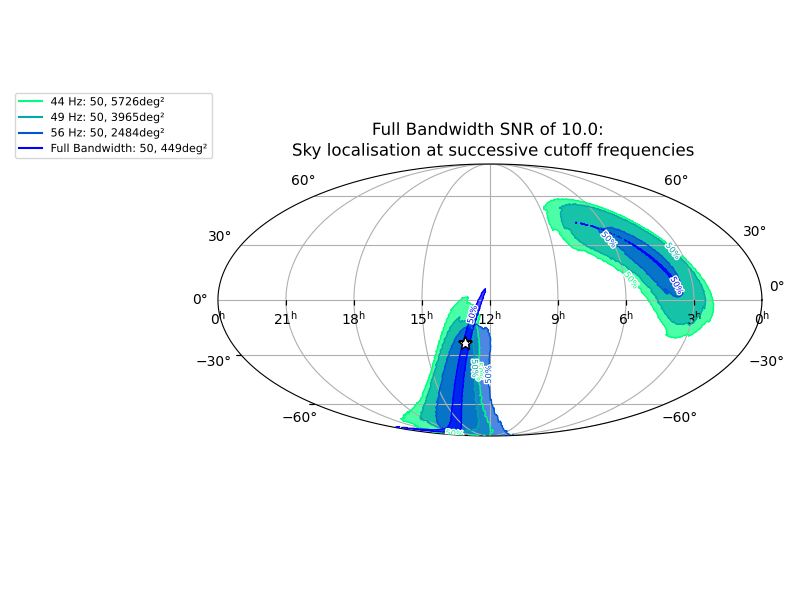
\includegraphics[width=\textwidth]{images/6_earlywarning/localisation/10SNR_multiple.png}
    \caption{}
    \label{fig:ew_10SNR_multiple}
\end{figure}
%
\begin{figure}
    \centering
    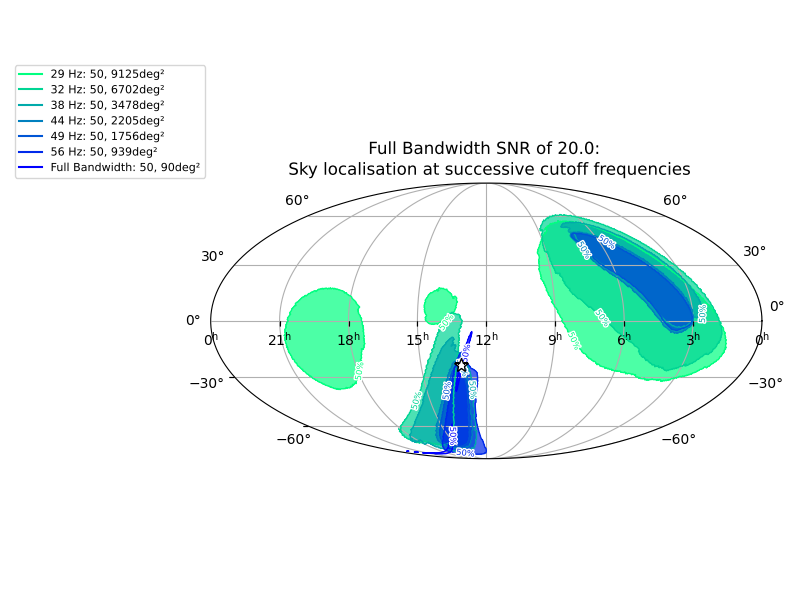
\includegraphics[width=\textwidth]{images/6_earlywarning/localisation/20SNR_multiple.png}
    \caption{}
    \label{fig:ew_20SNR_multiple}
\end{figure}
%
\begin{figure}
    \centering
    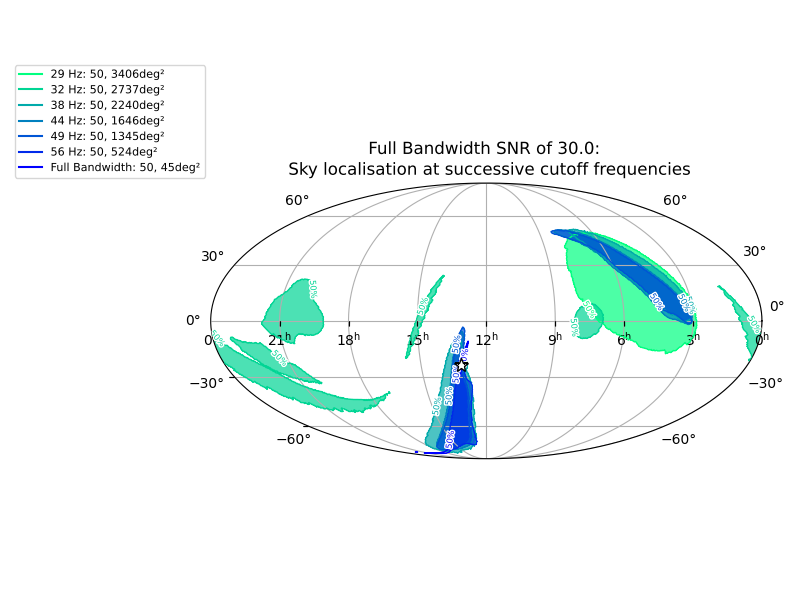
\includegraphics[width=\textwidth]{images/6_earlywarning/localisation/30SNR_multiple.png}
    \caption{}
    \label{fig:ew_30SNR_multiple}
\end{figure}
%
\begin{table}
    \centering
    \begin{tabular}{|l|c|c|c|}
        \hline
        \textbf{Final SNR} & \textbf{10} & \textbf{20} & \textbf{30} \\ \hline
        \textbf{Sky map} & 
        Figure~\ref{fig:ew_10SNR_multiple} &
        Figure~\ref{fig:ew_20SNR_multiple} &
        Figure~\ref{fig:ew_30SNR_multiple} \\ \hline
        \textbf{Frequency} & \multicolumn{3}{|c|}{\textbf{Localization accuracy} (50\% credible area)} \\ \hline
        29 Hz & Not detected    & 9125 deg$^2$ & 3406 deg$^2$ \\ \hline
        32 Hz &  & 6702 deg$^2$ & 2737 deg$^2$ \\ \hline
        38 Hz &  & 3478 deg$^2$ & 2240 deg$^2$ \\ \hline
        44 Hz & 5726 deg$^2$ & 2205 deg$^2$ & 1646 deg$^2$ \\ \hline
        49 Hz & 3965 deg$^2$ & 1756 deg$^2$ & 1345 deg$^2$ \\ \hline
        56 Hz & 2484 deg$^2$ & 939 deg$^2$  & 524 deg$^2$ \\ \hline
        1024 Hz & 449 deg$^2$ & 90 deg$^2$   & 45 deg$^2$ \\ \hline
    \end{tabular}
    \caption{Table with Final SNR, Distance, Sky map, Frequency, and Localization accuracy (50\% credible area)}
    \label{tab:ew_inj_skymaps}
\end{table}
%
It is the case, especially for the low SNR signal, that the injection at every final frequency cutoff. Figure~\ref{fig:ew_10SNR_multiple} is missing the \verb|29, 32| and \verb|38| Hz events. It is very clear to see in table~\ref{tab:ew_inj_skymaps} that a higher SNR directly translates to a better sky localisation. The 30 SNR injection has been constrained sky maps at all frequencies.

DESCRIBE THE SKY MAPS AND THE CONTOUR INTERVALS. 50\% REFERS TO THE SMALLEST AREA ON THE SKY, MINIMIZED. FIND OUT HOW THIS IS DONE. 

\section{Injection Runs in Offline}

To investigate the efficacy of the early warning search I performed an injection campaign very similar to the injection campaigns done in the previous chapters, (ARCHENEMY), (PYCBCLIVE). This time using an injection set I generated myself to include exclusively signals that should be seen by the early warning search, as opposed to the premade rates and populations injection sets.

\subsection{Injection Set \& Data}

The injection set contains 32,604 unique injections placed every $\sim100$ seconds, encompassing 3,456,000 seconds or exactly 40 days worth of data. The parameters which vary by injection and the ranges in which they vary can be seen in table~\ref{6:tab:ew_inj_params}.
%
\begin{table}[ht]
    \centering
    % \small
    \setlength{\tabcolsep}{4pt}
    \rowcolors{2}{white}{lightgray}
    \begin{tabular}{ccc}
        \toprule
        \multicolumn{3}{c}{\textbf{Variable Parameters}} \\
        \cmidrule(lr){1-3}
        \textbf{Parameter} & \textbf{Value Range} & \textbf{Prior Distribution} \\
        \midrule
        Primary Mass, $m_1$ & 1.0 - 3.0 [$M_{\odot}$] & uniform \\
        Secondary Mass, $m_2$ & 1.0 - 3.0 [$M_{\odot}$] & uniform \\
        Primary Spin z-component, $spin1z$ & -0.05 - 0.05 & uniform \\
        Secondary Spin z-component, $spin2z$ & -0.05 - 0.05 & uniform \\
        Distance, $r$ & 10 - 1000 [$Mpc$] & uniform radius \\
        Phase, $\phi_{c}$ & - & uniform angle \\
        Inclination, $\iota$ & - & sin angle \\
        Polarization, $\psi$ & - & uniform angle \\
        Right Ascension, $\alpha$ & - & uniform sky \\
        Declination, $\delta$ & - & uniform sky \\
        \bottomrule
        \multicolumn{3}{c}{\textbf{Static Parameters}} \\
        \cmidrule(lr){1-3}
        \textbf{Parameter} & \textbf{Value} & \textbf{} \\
        \midrule
        Waveform Approximant & IMRPhenomXAS & \\
        Lower Frequency, $f_{lower}$ & 17 [$Hz$] & \\
        Reference Frequency, $f_{ref}$ & 17 [$Hz$] & \\
        \bottomrule
    \end{tabular}
    \caption{Caption text goes here}
    \label{6:tab:ew_inj_params}
\end{table}
%
These injections are made into simulated noise with no non-Gaussian artefacts or non-stationarity and a constant PSD. The distances generated for each injection are re-scaled after the initial injection set has been created to ensure a uniform SNR distribution of the signals between 12 and 60. Therefore the distances might not be exactly uniform in radius and the injection set should be thought to be distributed uniformly in SNR instead.

\subsection{Results}

Each injection has the potential to be seen by six different templates and therefore we might expect to see exactly six times the number of injections in the data. However, for the very low final frequency templates in the bank (29Hz) these would require at least 4 (DOUBLE CHECK) SNR (the SNR threshold for detection) to be accumulated in a very small frequency window, which is very unlikely for the 12 SNR injections but possible for our 60 SNR injections. (CHECK THIS TO SEE WHAT THEY ACTUALLY FOLLOW, MINIMUM SNR FOR 29Hz DETECTION)

Another reduction in the number of candidates found will be caused by a very short time gap between final frequencies 49Hz and 56Hz. The evolution of the gravitational wave signals inspiral increases over time and therefore these two frequencies might be found within a stride and therefore one will be skipped. These two effects will cause a reduction in the total number of candidates seen by this injection test.

The total number of candidates found for all injections is (NUMBER). 

PyCBC Live outputs the candidates found during the search and outputs the time of coalescence of the non-truncated template. Therefore, even if a 29Hz template finishes many seconds before time of coalescence of the gravitational wave signal, we can collect all of the candidates associated with an injection by comparing injection time and time of coalescence of candidates. We look for candidates with a time of coalescence within +-0.5 seconds of the injection time, this ensures that we are looking for candidates which have all been predicted to end in the same search stride.

Figure~(REF) shows a histogram of the number of candidates found per injection. (INSERT THE FIGURE)

\section{Identified Problems}

The purpose of performing this experiment is to see where the early warning search is lacking and could be improved in the future to allow for greater chance of properly detecting these exceedingly rare events when they occur for real.

We have identified some problems with the early warning search during this injection test which we will describe here, where possible I will indicate whether these problems can be solved as of right now or if more work needs to go into developing solutions in the PyCBC Live search. Alongside this, some of these problems are expected and the solutions would harm the search and so are left as is.

\subsection{Low significance candidates}

As with any search, the template bank can match on Gaussian noise in the data and produce low significance candidates that typically only upload a single candidate per injection. These can also end at a similar time of coalescence to another found injection and so can appear in the results as belonging to an injection when they are entirely independent and made of noise.

These can be treated by GraceDB in post-upload and disregarded quite quickly when further candidate uploads from higher final frequency templates have not been made. However, this is another consequence of the low-latency matched filter searches. Figure~REMOVED shows an example of an injection having another associated 29Hz candidate which ends at a similar time of coalescence but is on an entirely different track to the injection's other found candidates.
%
\begin{figure}
       \centering
    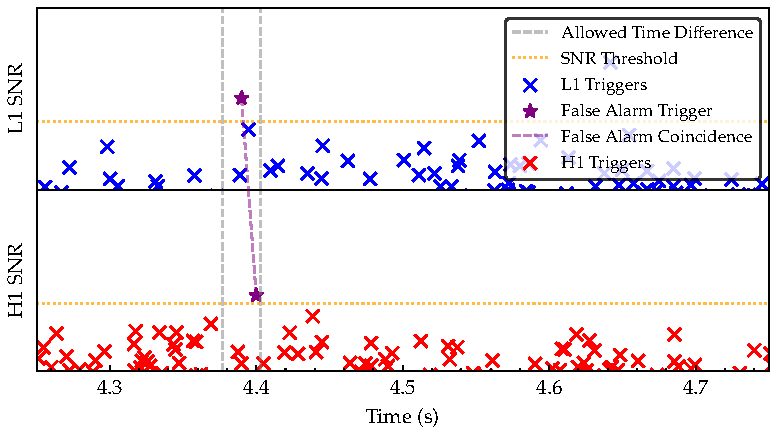
\includegraphics[width=\textwidth]{images/6_earlywarning/identified-problems/low_sig_cands.pdf}
    \caption{}
    \label{6:fig:low_significance_candidates}
\end{figure}
%

\subsection{Missing frequencies in signal evolution}

Injections which are missing frequencies are those that might seem to skip a frequency candidate, for example, progressing through from 32Hz to 38Hz, missing a 44Hz candidate and then finding a 49Hz and 56Hz candidate. We want to understand why the 44Hz candidate was missed. The smooth progression of frequency candidates could be used in the future as a measure of how real and event is, so to miss a candidate for a non-astrophysical reason might reduce our sensitivity.

There is a simple explanation for some events which is that the progression through to the higher frequencies might simple be too short for the search to identify a separate candidate. For the higher mass templates there might be few seconds between candidates. Others there is a clear problem and it is useful to understand why this has happened.
%
\begin{figure}
       \centering
    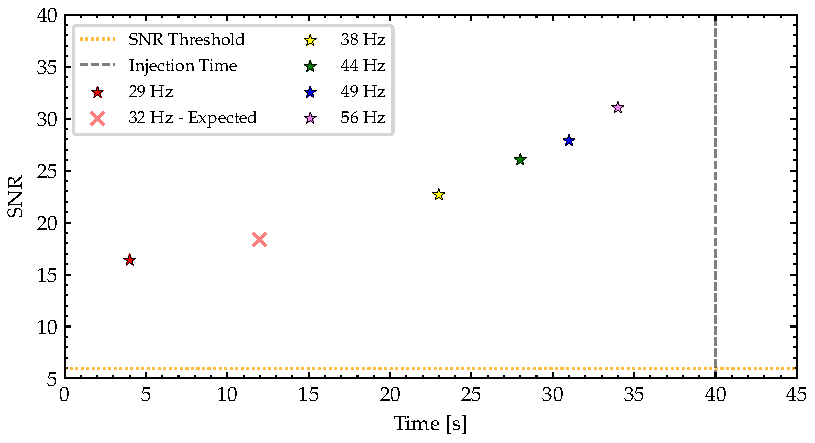
\includegraphics[width=\textwidth]{images/6_earlywarning/identified-problems/missing_freqs.pdf}
    \caption{}
    \label{6:fig:missing_frequencies}
\end{figure}

\subsection{Non-monotonic SNR increases}

As a gravitational wave signal passes through the detectors we can match more and more of it to the gravitational wave template and can expect to see a higher and higher SNR. Therefore, for a specific gravitational wave signal we would expect an increasing SNR from each candidate corresponding to each final frequency in our template bank. We look at the network SNR from each candidate corresponding to a gravitational wave event and we can see if any consecutive candidates have a lower SNR from the previous candidate, an unexpected behaviour.

We find that 1398 injections have a non-monotonically increasing SNR at some point within their evolution. To prevent the effects of small noise fluctuations we compare the SNRs from the two candidates and assess whether there is a greater than 5\% drop in SNR. For example, if the 38Hz candidate has an SNR of 10, the 44Hz candidate must have an SNR of less than 9.5 to be counted as a non-monotonic injection.
%
\begin{figure}
       \centering
    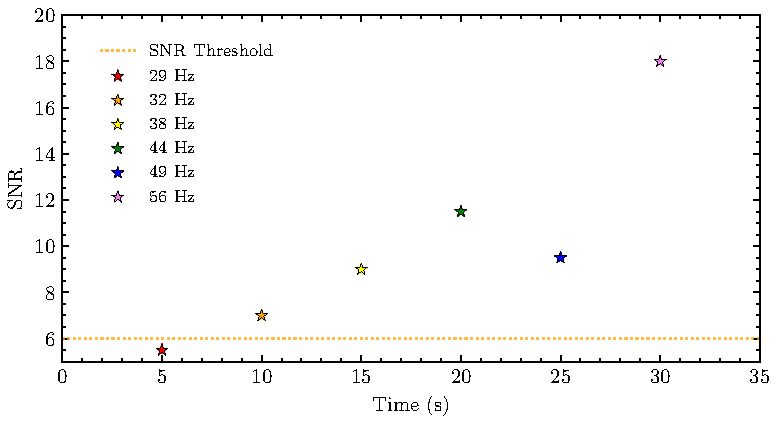
\includegraphics[width=\textwidth]{images/6_earlywarning/identified-problems/non_mono_snr.pdf}
    \caption{}
    \label{6:fig:non-monotonic-snr}
\end{figure}
%
To understand why these are happening, we have to look at the components that not only give us the SNR--the template and the data-- but also the ranking statistic, which might favour a slightly lower SNR template due to other properties of the noise. For example, the same template for the 38Hz and 44Hz candidates might give a monotonic increase in SNR but, a different template with a lower SNR for the 44Hz candidate might be more highly preferred event.

\subsection{Candidates across search boundaries}
%
\begin{figure}
       \centering
    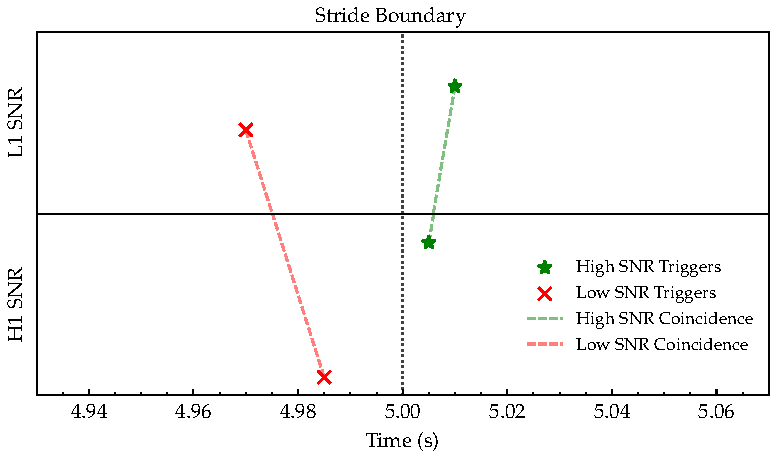
\includegraphics[width=\textwidth]{images/6_earlywarning/identified-problems/cands_across_bounds.pdf}
    \caption{}
    \label{6:fig:candidates_across_boundaries}
\end{figure}
%
The early warning search operates on a one second stride, meaning every single second the template bank is matched filtered with the data to discover any gravitational wave signals. In some cases the SNR of a template match filtered with the data will be above the SNR threshold in one second and again above the SNR threshold in the next second.

There are two scenarios for this case, the first second has a lower SNR than the following second: in this case, there will be two candidates uploaded to GraceDB with the same template and roughly the same time of coalescence (within 0.5 seconds) where one has a higher SNR than the other. We want to reduce the amount of lag from detection to upload so there is no possibilty of keeping a 'buffer' of candidates to hold whether a higher SNR candidate will occur in the next second and this will be a scenario that will just happen.

The second scenario is the same happening but the other way round, the first candidate has a higher SNR than the candidate in the following second. In this case we can happily upload the first candidate to GraceDB and then keep track of the uploaded candidates and prevent the upload of the second candidate if it has a lower SNR. This is already implemented in PyCBC Live for the single detector search and can be easily changed to be used for the early warning search too in the future.

In figure~REMOVED you can see a great example of this happening for one of our injections. It appears that multiple candidates have been created for multiple final frequency templates, these candidates have different SNRs but are found with the same template and the same time of coalescence for the injection.

\subsection{Triggers across search boundaries}
%
\begin{figure}
       \centering
    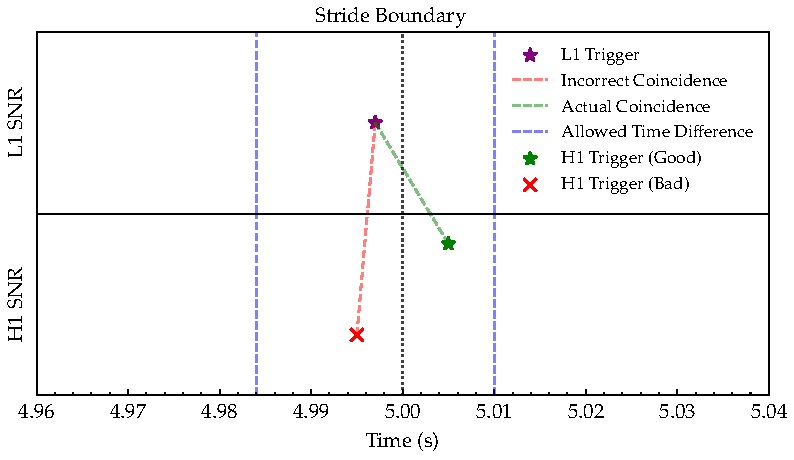
\includegraphics[width=\textwidth]{images/6_earlywarning/identified-problems/trigs_across_bounds.pdf}
    \caption{}
    \label{6:fig:triggers_across_boundaries}
\end{figure}
%
The early warning search operates using coincidences across detectors which have a phase-time consistency test included in the coincident detection ranking statistic. The time portion of this test allows for a light travel time (plus a small buffer) between triggers in different detectors. This light travel time can mean that triggers in separate detectors for the same gravitational wave injection can fall on different sides of a second stride. Therefore the early warning search will create two candidates with the highest SNR trigger in the first detector with two other triggers for the second detector in two separate second strides.

This is unfortunately unavoidable, we need the light travel time in the ranking statistic and this can straddle two strides. Tracking candidates uploaded in the previous second and holding an upload if the SNR is lower in the second second would still help but the same trigger from a single detector will be uploaded twice.

\section{\label{6:sec:stories}Investigating Individual Injections}

\section{\label{6:sec:potential-improvements}Potential Improvements}

While I am not including the improvements that are suggested here into the early warning search, due to time constraints, I will delve into some of the improvements that can be made and the positives and negatives of their effect upon the search.

\subsection{\label{6:subsec:ranking-statistic}Additions to the Ranking Statistic}

The ranking statistic, as mentioned in previous chapters, is the way in which we can evaluate the likelihood of a particular candidate being 'real'. Therefore, if we include more and more components into the ranking statistic, we can build up a more confident picture of what determines the realness of a candidate and whether we should share this candidate with the wider research community.

The current ranking statistic used by the early warning search is very very simple, in the single detector triggers it is a simple ranking of `newsnr' where the chi squared tests are used to determine if the correct amount of power is located in each bin of the template. For the coincident ranking statistic we used `phasetd' which is another simple check of phase and amplitude consistency between detectors in the time domain.

We have two careful consideration with regards to the ranking statistic. Number 1, computation time and avoiding introducing any lag into the early warning search. The early warning search has a stride length of one second, if any complicate computational steps are added to the ranking statistic we might risk delaying any detected early warning candidates and defeating the purpose of the search. Number 2, eliminating potential candidates before we send them out. No ranking statistic is perfect and the resulting quantitative analysis from the ranking statistic, the false alarm rate, is cut off at a human chosen number (typically one or two per year). Therefore, if we introduce more and more complicated components to the ranking statistic we might risk eliminating early warning candidates which don't meet the PyCBC threshold of a confident event but, other non-IGWN people might take that risk and perform their observations or analyses using our non-confident predictions. Therefore we might actually want to either keep our ranking statistic fairly simple, to not lose these rare events, or lower our threshold when using a complicated ranking statistic so that we still disperse these events but with a big asterisk that we do not think they're real and might fall below someone's threshold.

If we wanted to make some improvements to the ranking statistic we can consider including some early warning specific information which we would know at the time of the search. This is either historical information based on the previous results produced by the early warning search, something similar to the template fits used in offline and the full bandwidth live search, or maybe even an astrophysical analysis of what we expect to see based on a population model, something like the KDE statistic (I think??).

Real time information that could be used in the search pertains to the state of the detector at that very time, inclusion of iDQ and DQ, it could also include the detected candidates that have already been found and are being kept in a rolling buffer. We do expect that for a real gravitational wave signal that can be found in early warning, to see a cascade of events uploaded with subsequent frequencies getting higher and higher. We could check if any previous frequencies were uploaded, or in posterity whether any further frequencies were uploaded. If a candidate has been found first at 38Hz, does this mean we missed a 29Hz and a 32Hz signal or were these too quiet? Can we spin up a small job to do a deep dive on whether these lower frequencies are in-fact there? There are many small changes that can be made to the early warning search to iteratively improve upon it and make it more robust and confident in detecting these rare events.

\subsection{More Frequency Truncations per Template}
We currently have five frequency truncations per template in our bank. This is to prevent a massive amount of templates in the bank and is a good balance for shorter templates which might transition between frequency truncations faster than the search stride time when reaching higher frequencies.

We could produce a template bank with a number of different configurations and requirements:
- Greater number of frequency truncations for all templates
- Template dependent frequency truncations, longer duration templates will have more frequency truncations
- Equal truncations per template but sigma dependent spacing
- Time before merger spacing of templates, 1 template every 3/4/5 seconds or something. Or 8 templates per duration

\subsection{Great parameter distribution in template bank}
The distribution of template parameters is conservative in the early warning search. We only want to find and report on signals that have a potential electromagnetic counterpart however our template bank could be too conservative and by allowing a greater parameter distributions of templates we could discover some templates on the edge of the bank with a greater SNR or templates that previously we wouldn't have seen.

To test a larger template bank we would need to produce an injection set containing a larger number of signals that we might consider EM bright, recent literature has highlighted previously unknown signals that could have EM counterparts~SOURCE SOURCE SOURCE.

\subsection{Adding Spins to the Template Bank}
Currently the template bank is limited to aligned 0 spin templates. We tested the search with an injection set of slightly spinning templates and this spin will not be seen by the early warning search. It is known that neutron stars have theoretical spins up to +-0.4 so there is a potential for us to be missing spinning neutron star signals and therefore precessing signals in our search. While precessing signals are more difficult to see due to difficulties in including the many more parameters requires this search is very light weight currently and more computing power could be added to balance out the lag increase from introducing more complicated template banks to the search.

\subsection{Approximants with greater physics}
Due to the small number of templates and them being only generated once for the live search we might be able to use a more expensive template model which includes physics which can capture some unique properties of low mass signals like tidal deformation or orbital eccentricity, using a better equation of state, higher order modes or high order PN terms.






%%%%%%%%%%%%%%%%%%%%%%%%%%%%%%%%%%%%%%%%%%%%%%%%%%%%%%

\section{Problems Faced when producing Injection Data}

One of the problems experienced while doing the data analysis of this project is an issue caused by the method of creating the data initially. The PyCBC function used was \emph{pycbc\_condition\_strain} which takes an input for the power spectrum density of the noise you with to simulate. We used an analytical PSD (NAME, REF, CITE) which produced discontinuities at the boundaries between our data segments and therefore negative effects on the matched filtering being performed by the live search. An example of one of these discontinuities and an injection missing some candidates can be seen in figure~REMOVED.
% %
% \begin{figure}
%        \centering
%     \includegraphics[width=\textwidth]{}
%     \caption{}
%     \label{fig:ew_boundary_problem}
% \end{figure}
% %
The bug can be explained by the analytical PSD not cutting off naturally when tending towards 0Hz and instead takes on values incompatible with a real PSD. This 'bug' has since been reported and a user-based solution has been found, to include a new argument to condition strain to perform a highpass on all frequencies below 10Hz. Unfortunately we did include a highpass argument on the data originall when creating the data but it was the wrong one!

Since discovering this boundary issue the same data has been re-created with the same PSD but the correct highpass argument has been given and therefore the boundary issue has been resolved and we have re-performed the initial data analysis with the new data.


\section{Existing Limitations}

\subsection{Computational Limitations}

The early warning search is heavily optimized to the point it runs on a single dedicated machine with $10$ processes and $2$ threads per process. Just as the with full bandwidth search, the template bank is parallelised over these processes using MPI so each process will be performing the matched filter for only a few hundred templates before the message passing interface receives all the results and the coicidences are found by the rank 0 process. The search can be badly affected by other processes running on the same machines so this machine is exclusively used by the PyCBC Live early warning search.

The search can suffer heavily from other non-PyCBC processes such as file storage, data frame delivery or GraceDB uploads. These can be mitigated slightly with reserved local storage on the dedicated machine or subprocess multiprocessing for the GraceDB uploads so the search isn't waiting on GraceDB to continue processing, especially at times where multiple events are being uploaded for a single signal and across multiple searches from other pipelines.

Another consideration and computational limitation is the limit in introducing new computationally complex processes to the search that might introduce lag to individual processes. Potential changes to the ranking statistic could be challenging to implement without slowing down individual processes or the coincidence rank 0 process. With a data stride of one second we need to be sure that the data processing for the current second is completed before the next second of data arrives or we will slowly build up a debt of data which the search can never get on top of.

\subsection{Physical Limitations}

The template bank does not include any spins on the templates thereby neglecting any effects on the waveform or from precession, however, it is unlikely to see precession at such low frequencies due to the effect becoming more pronounced over increasing numbers of orbits.

Electromagnetically bright events are very rare in the LVK regime, as of May 2024 only (NUMBER) out of (TOTAL NUMBER) events are within our template bank range, and of those only (NUMBER) have been observed with electromagnetic counterparts.

